\chapter{Mitigate Fingerprinting of Honeypots}
\label{chap:fingerprinting}

\section{Fingerprinting Cowrie}

Attackers have a strong motivation to reveal honeypots before launching an attack.
Without any protection attackers would disclose their methods, and thus, newly developed attacks would become useless.
As shown in \autoref{chap:cloud-security}, attackers do try to get information about the host system.
\citet{vetterl2020} discussed various methods of fingerprinting, however, executing commands in a login shell and examining the response leaves precarious information to the honeypot itself.
In his work he evaluated methods to detect honeypots at the transport level.
As stated, the value of a honeypot would be merely zero if a detection on transport level would work.
He presents fingerprinting methods for SSH, Telnet, and HTTP/Web.
Due to the complexity of each method, we focus on SSH fingerprinting with the honeypot Cowrie.
The idea to detect SSH honeypots is to look for deviations in the response.
Therefore, \citet{vetterl2020} sends a set of probes $P = \{P_1, P_2, \dots, P_n\}$ to a given set of implementations of a network protocol $I = \{I_1, I_2, \dots, I_n\}$ and stores the set of responses $R = \{R_1, R_2, \dots, R_n\}$.
For the given set of responses he calculated the cosine similarity coefficient $C$.
Goal is to find the best $P_i$ where the sum of $C$ is the lowest.
\autoref{fig:draft-cosine-similarity} presents these steps.

Cosine similarity outputs the similarity between vectors of numerical attributes.
In text semantics it is widely used to measure the similarity of sets of information such as two sentences.
\citet{vetterl2020} outlines that it can be used in \enquote{traffic analysis to find abnormalities and to measure domain similarity}.
Mathematically, it computes the angle between two vectors.
For each set of information $A$, we create a vector $D_A$.
Referring to our use case with SSH, we use the response from the server as information $A$.
If $\theta$ is the angle between $D_A$ and $D_B$, then:

\begin{equation} \label{eq:cosine-similarity}
    \cos \theta = \frac{D_A \cdot D_B}{\|D_A\| \|D_B\|}
\end{equation}

where \enquote{$\cdot$} is the dot product obtained by:

\begin{equation}
    D_A \cdot D_B = \sum_{i=1}^{n} (D_{A_i} \times D_{B_i})
\end{equation}

and $\|D_A\|$ (resp. $\|D_B\|$) is the Euclidean norm, obtained by $\sqrt{\sum_{i=1}^{n} D_{A_i}^2}$ (resp. $\sqrt{\sum_{i=1}^{n} D_{B_i}^2}$).
The values of vectors are non-negative. The similarity between items is the value $\cos \theta$, $\cos \theta = 1$ indicates equality.

\begin{figure}[ht]
    \centering
    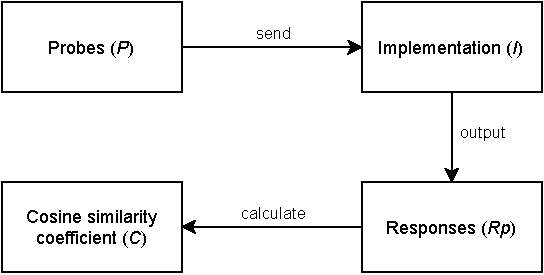
\includegraphics{figures/vetterl_concept.pdf}
    \caption[(derived from \cite{vetterl2020})]{Outline to }
    \label{fig:draft-cosine-similarity}
\end{figure}

In order to find the best $P_i$ for SSH, \citet{vetterl2020} first created different SSH version strings based on the format \verb|SSH-protoversion-swversion SP comment crlf|.
He used different lower and upper case variations, 12 different protoversions ranging from $0.0$ to $3.2$, swversion set to OpenSSH or empty string, comment set to FreeBSD or empty string, and crlf to either \verb|\r\n| or empty string.
In total, summing up to 192 client version strings.
Second, he created different \verb|SSH2_MSG_KEXINIT| packets with 16 key-exchange algorithms, 2 host key algorithms, 15 encryption algorithms, 5 MAC algorithms and 3 compression algorithms.
In total, he sent \numprint{58752} \verb|SSH2_MSG_KEXINIT| packets.
Combining them with the 192 client versions, he ended up sending \numprint{157925376} packets.
The version string \verb|SSH-2.2-OpenSSH\r\n| and the \verb|SSH2_MSG_KEXINIT| packet including ecdh-sha2-nistp521 as key-exchange algorithm, ssh-dss as host key algorithm, blowfish-cbc as encryption algorithm, hmac-sha1 as mac algorithm and zlib@openssh.com as compression algorithm, with the wrong padding results in the lowest cosine similarity coefficient $C$.
\autoref{tab:cosine-similarity} presents the cosine similarity of OpenSSH, Twisted, and Cowrie.
As it outlines, Cowrie responses are not close to OpenSSH.
Thus, distinguishing Cowrie from OpenSSH with SSH packets is feasible.
Moreover, \citet{vetterl2020} performed an Internet-wide scan and detected $2021$ Cowrie honeypots.
These results indicate the weak link 

\begin{figure}[ht]
    \centering
    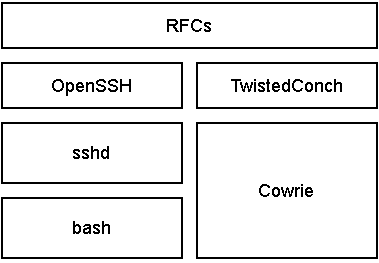
\includegraphics{figures/cowrie-openssh.pdf}
    \caption[Architecture of OpenSSH and Cowrie]{Architecture of OpenSSH and Cowrie. OpenSSH and TwistedConch have subtle differences.}
    \label{fig:cowrie-openssh}
\end{figure}

\citet{vetterl2020} states that current low- and medium-interaction honeypots have a generic weakness due to the underlying off-the-shelf libraries.
Cowrie is based on TwistedConch, a Python 2/3 library that implements the SSH protocol.
Any bash command and its response are tweaked by Cowrie, and thus, resulting in a discrepancy to OpenSSH.
For example, Cowrie version $1.1.0$ missed \verb|tftp| and came with version $1.2.0$.
So, it is continuous struggle of adding to commands to avoid early disclosures of Cowrie.


\begin{table}
    \caption{Overview of the cosine similarity of OpenSSH, Cowrie, and Twisted.}
    \begin{tabular}{lc|cccccccccc}
    \toprule
                   &   & A & B      & C      & D      & E      & F      & G      & H      & I      & J      \\
    \hline
    OpenSSH 6.6    & A & - & $0.98$ & $0.98$ & $0.94$ & $0.94$ & $0.42$ & $0.78$ & $0.79$ & $0.79$ & $0.79$ \\
    OpenSSH 6.7    & B &   & -      & $0.98$ & $0.98$ & $0.98$ & $0.41$ & $0.80$ & $0.81$ & $0.81$ & $0.80$ \\
    OpenSSH 6.8    & C &   &        & -      & $0.96$ & $0.96$ & $0.42$ & $0.78$ & $0.79$ & $0.79$ & $0.79$ \\
    OpenSSH 7.2    & D &   &        &        & -      & $0.98$ & $0.42$ & $0.80$ & $0.80$ & $0.80$ & $0.80$ \\
    OpenSSH 7.5    & E &   &        &        &        & -      & $0.42$ & $0.78$ & $0.79$ & $0.79$ & $0.79$ \\
    \\
    \cline{1-2} \cline{8-12}
    \\
    Twisted 15.2.1 & F &   &        &        &        &        & -      & $0.50$ & $0.51$ & $0.51$ & $0.52$ \\
    \\
    \cline{1-2} \cline{9-12}
    \\
    Cowrie 96ca2ba & G &   &        &        &        &        &        & -      & $0.98$ & $0.98$ & $0.98$ \\
    Cowrie dc45961 & H &   &        &        &        &        &        &        & -      & $0.99$ & $0.99$ \\
    Cowrie dbe88ed & I &   &        &        &        &        &        &        &        & -      & $0.99$ \\
    Cowrie fd801d1 & J &   &        &        &        &        &        &        &        &        & -      \\
    \bottomrule
    \end{tabular}
    \label{tab:cosine-similarity}
\end{table}

\section{Disguising Cowrie}

Proxying SSH commands to Cowrie helps to block any fingerprinting activities.


\section{Experiment}

\begin{figure}
    \lstinputlisting[language=bash, caption={OpenSSH connection attempt with probed SSH packet}, label={lst:ssh-openssh}]{listings/ssh-openssh.txt}
\end{figure}

\begin{figure}
    \lstinputlisting[language=bash, caption={Cowrie connection attempt with probed SSH packet}, label={lst:ssh-cowrie}]{listings/ssh-cowrie.txt}
\end{figure}

\begin{figure}
    \lstinputlisting[language=bash, caption={Disguised Cowrie connection attempt with probed SSH packet}, label={lst:ssh-cowrie-fixed}]{listings/ssh-cowrie-fixed.txt}
\end{figure}

%So would it be ok if you take a picture of the IBM box inside the shipping box  with my delivery details and timestamp? And additionally, a picture of the sealed shipping box with the shipping note from DHL.
%I guess that would be sufficient for me.